%!TEX root = ../../thesis.tex

The discovery of the Higgs boson appears to ``complete'' the SM in the most minimal way, 
with no significant deviations from predictions observed. That its 
\HepProcess{\PHiggs\PW\PW} and \HepProcess{\PHiggs\PZ\PZ} couplings agree with 
expectations confirms that the Higgs mechanism underlies electroweak symmetry breaking. 
That its fermionic couplings are proportional to mass supports that fermion masses are 
generated by Yukawa interactions.

In Sections~\ref{sec:implications:ewfit} and \ref{sec:implications:vacuum}, the 
discovered Higgs boson shall be interpreted assuming that the SM is valid up to the 
Planck energy scale (at which point gravity becomes strong and dominates phenomenology). 
Then, \Section~\ref{sec:implications:hierarchy} considers why the observed particle might 
indicate that new physics should be observed at lower scales.



\subsection{Global electroweak fit}
\label{sec:implications:ewfit}

In \Section~\ref{sec:prior_constraints:ew_fits}, a global fit of electroweak data was 
used to motivate a low mass Higgs boson. The discovery of the Higgs boson and the 
measurement of its mass overconstrains the electroweak theory, allowing a test of its 
validity. 

The updated fit exhibits a $p$-value of 0.176, corresponding to a deviation from the 
Standard Model of significance $1.35\sigma$ \cite{Gfitter:2013}. Thus, the experimental 
data included in the fit are consistent with electroweak theory. The pulls of individual 
fit parameters are shown in \Figure~\ref{fig:concl:ewfit_pulls}; the dominant tension is 
unrelated to \mH. The measurement of \mH does cause some tension with the measured \mW 
and $m_{\Ptop}$, which are sensitive to \mH through loop corrections.

\begin{figure}[p]
	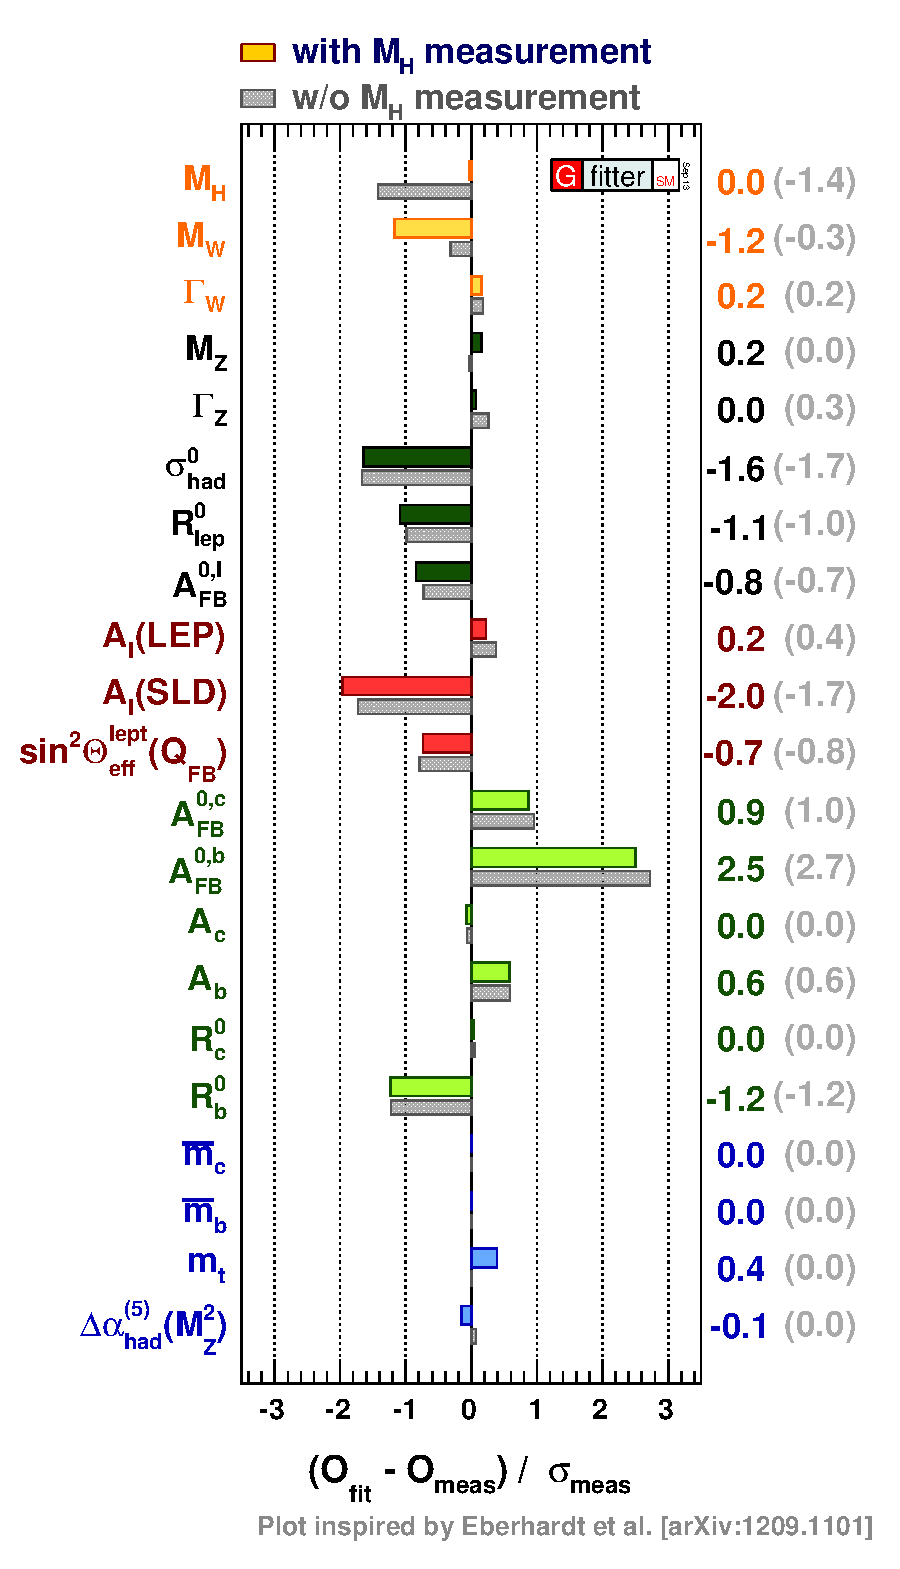
\includegraphics[width=\mediumfigwidth]{tex/conclusions/ewfit_pulls}
	\caption{Pull values of the electroweak fit parameters, with (colour) and without 
	(grey) the \mH measurement included \cite{Gfitter:2013}. The pull value is the 
	deviation of the fitted value from the experimental measurement, in units of the 
	experimental uncertainty.
	With kind permission from Springer Science and Business Media.}
	\label{fig:concl:ewfit_pulls}
\end{figure}



\subsection{Vacuum stability}
\label{sec:implications:vacuum}

In \Section~\ref{sec:prior_constraints:theory}, theoretical arguments were used to 
constrain \mH under the assumption that the Standard Model is valid up to the reduced 
Planck scale \unit{$\bar{\Lambda}_{\text{P}}~\about~10^{18}$}{\GeV}. Requiring the Higgs 
quartic coupling $\lambda$ remain perturbative implied \unit{$\mH < 175$}{\GeV}, while 
requiring the electroweak vacuum to remain a stable minimum implied 
\unit{$\mH > 129$}{\GeV} \cite{Ellis:2009}. 

The measurement of \unit{$\mH \approx 125$}{\GeV} excludes the stability of the SM vacuum at 
98.6\% CL \cite{Degrassi:vacuum}. However, a potential barrier separates the vacuum in 
which the Universe currently resides and the true SM vacuum. The probability of quantum 
tunnelling through this barrier is sufficiently small that the lifetime of the Universe 
far exceeds its age. Thus, measurements suggest that we exist in a metastable vacuum (see 
\Figure~\ref{fig:concl:vacuum_stability}).

\begin{figure}[t]
	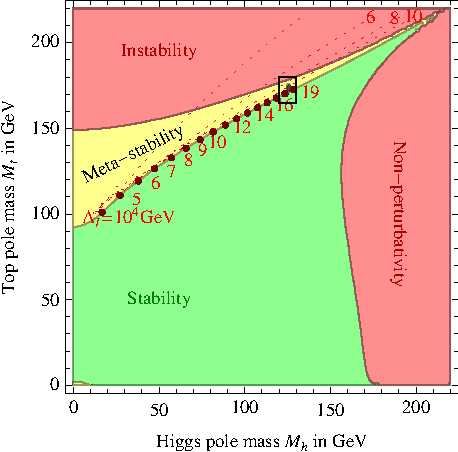
\includegraphics[width=0.48\textwidth]{tex/conclusions/vacuum_stability}
	\hfill
	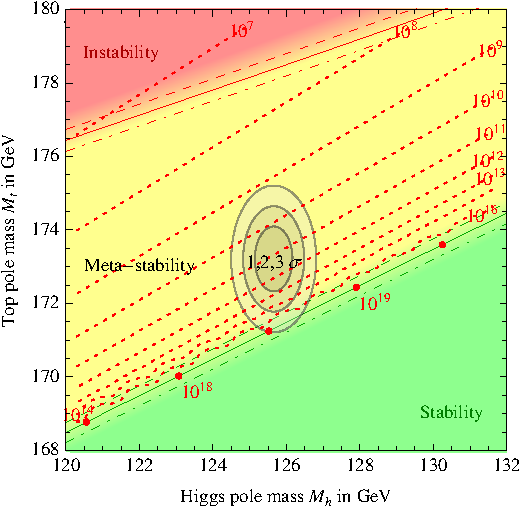
\includegraphics[width=0.49\textwidth]{tex/conclusions/vacuum_stability_zoom}
	\caption{Phase diagram of the Standard Model, expressed in terms of \mH and 
	$m_{\Ptop}$ \cite{Degrassi:vacuum}. The phases correspond to stable, metastable and 
	unstable vacuum states and a non-perturbative Higgs quartic coupling $\lambda$, 
	assuming that the scale at which new physics is introduced is 
	\unit{$\Lambda_{\text{NP}} = \Lambda_{\text{P}}~\about~10^{19}$}{\GeV}. Dotted lines 
	indicate the scale at which the instability phase transition occurs. A zoomed version 
	(right) elucidates the experimentally measured situation.}
	\label{fig:concl:vacuum_stability}
\end{figure}

The fact that experimental measurements place the Universe very close to the critical 
boundary for vacuum stability means that $\lambda$ and $\beta_{\lambda}$ are both very 
close to zero at the instability scale. The potential significance of this observation is 
an active area of theoretical research. One interesting idea also uses the scalar 
nature of the Higgs boson to lend credence to slow-roll models of cosmic inflation with 
the Higgs boson acting as the inflaton. However, minimal configurations of such models 
may fail to predict the power spectrum of anisotropies observed in the cosmic microwave 
background \cite{Isidori:2007,DeSimone:2009}.



\subsection{The hierarchy problem}
\label{sec:implications:hierarchy}

The Higgs boson acquires a mass through oscillations about the non-zero vacuum 
expectation value of the Higgs field. However, this tree-level mass is subject to loop 
corrections containing massive particles; the top quark loop dominates, though the \PW, 
\PZ and Higgs bosons also contribute significantly. Similar corrections to \mW and 
$m_{\Ptop}$ were used to constrain \mH in \Section~\ref{sec:prior_constraints:ew_fits}.

Such loop diagrams should in principle be calculated to infinitely high scale, introducing 
ultraviolet (UV) divergences. They can be calculated within the SM for scales up to 
\unit{$\Lambda_{\text{P}}~\about~10^{19}$}{\GeV}, but a theory of everything (ToE) would 
be needed above $\Lambda_{\text{P}}$. These corrections to \mH are quadratically 
divergent, and so the measured \mH can be schematically written as
\begin{equation}
	m_{\text{\PHiggs,physical}}^2 &= m_{\text{\PHiggs,bare}}^2 + \int\limits_{0}^{\Lambda_{\text{P}}} \text{SM loops} + \int\limits_{\Lambda_{\text{P}}}^{\infty} \text{ToE loops} \\
	&= m_{\text{\PHiggs,bare}}^2 + \ofOrder{\Lambda_{\text{P}}^2} + \int\limits_{\Lambda_{\text{P}}}^{\infty} \text{ToE loops} \,.
\end{equation}
The bare mass $m_{\text{\PHiggs,bare}}$ is not predicted by the SM, but when combined with 
the ToE loops it must largely cancel the $\ofOrder{\Lambda_{\text{P}}^2}$ term, leaving 
behind $m_{\text{\PHiggs,physical}}^2 = \parenths{\unit{125}{\GeV}}^2$. This requires the ToE to produce a 
fine tuning of 1 part in $\parenths{\Lambda_{\text{P}}/\mH}^2~\about~10^{34}$, which is 
highly unnatural.

One may ask why the hierarchy problem is specific to the Higgs boson, and the same fine 
tuning is not required for other particles. This is because corrections to the masses of 
other particles are only logarithmically divergent (rather than quadratically divergent); 
their masses are protected by gauge or chiral symmetries.

If new physics exists at a scale $\Lambda_{\text{NP}} \ll \Lambda_{\text{P}}$, say 
\ofOrder{\unit{1}{\TeV}}, the degree of fine tuning can be reduced dramatically. This is 
a primary motivation for many new physics models. Supersymmetry introduces a new symmetry 
between fermions and scalars, which protects \mH \cite{SUSY}. Technicolour regards the 
Higgs boson as a composite state \cite{Peskin:1997}. Models with extra dimensions 
assume that gravity is actually strong, but $\Lambda_{\text{P}}$ appears large because 
the gravitational flux is diluted in the extra dimensions \cite{extradimensions}.

Thus, the existence of the Higgs boson motivates new physics at a scale 
\ofOrder{\unit{1}{\TeV}}. However, no experimental evidence in support of the candidate 
models has been found at the LHC, and indeed many configurations have been excluded.

